\documentclass[11pt,a4paper]{article}
\usepackage[english,greek]{babel}
\usepackage[utf8]{inputenc}
\usepackage{nimbusserif}
\usepackage[T1]{fontenc}
\usepackage[left=1.50cm, right=1.50cm, top=2.00cm, bottom=2.00cm]{geometry}
\usepackage{amsmath}
\let\myBbbk\Bbbk
\let\Bbbk\relax
\usepackage[amsbb,subscriptcorrection,zswash,mtpcal,mtphrb,mtpfrak]{mtpro2}
\usepackage{graphicx,multicol,multirow,enumitem,tabularx,mathimatika,gensymb,venndiagram,hhline,longtable,tkz-euclide,tkz-euclide,tkz-tab,fontawesome5,eurosym,tcolorbox,tabularray}
\usepackage[explicit]{titlesec}
\tcbuselibrary{skins,theorems,breakable}
\newlist{rlist}{enumerate}{3}
\setlist[rlist]{itemsep=0mm,label=\roman*.}
\newlist{alist}{enumerate}{3}
\setlist[alist]{itemsep=0mm,label=\alph*.}
\newlist{balist}{enumerate}{3}
\setlist[balist]{itemsep=0mm,label=\bf\alph*.}
\newlist{Alist}{enumerate}{3}
\setlist[Alist]{itemsep=0mm,label=\Alph*.}
\newlist{bAlist}{enumerate}{3}
\setlist[bAlist]{itemsep=0mm,label=\bf\Alph*.}
\newlist{askhseis}{enumerate}{3}
\setlist[askhseis]{label={\Large\thesection}.\arabic*.}
\renewcommand{\textstigma}{\textsigma\texttau}
\newlist{thema}{enumerate}{3}
\setlist[thema]{label=\bf\large{ΘΕΜΑ \textcolor{black}{\Alph*}},itemsep=0mm,leftmargin=0cm,itemindent=18mm}
\newlist{erwthma}{enumerate}{3}
\setlist[erwthma]{label=\bf{\large{\textcolor{black}{\Alph{themai}.\arabic*}}},itemsep=0mm,leftmargin=0.8cm}

\newcommand{\kerkissans}[1]{{\fontfamily{maksf}\selectfont \textbf{#1}}}
\renewcommand{\textdexiakeraia}{}

\usepackage[
backend=biber,
style=alphabetic,
sorting=ynt
]{biblatex}

\DeclareTblrTemplate{caption}{nocaptemplate}{}
\DeclareTblrTemplate{capcont}{nocaptemplate}{}
\DeclareTblrTemplate{contfoot}{nocaptemplate}{}
\NewTblrTheme{mytabletheme}{
\SetTblrTemplate{caption}{nocaptemplate}{}
\SetTblrTemplate{capcont}{nocaptemplate}{}
\SetTblrTemplate{contfoot}{nocaptemplate}{}
}

\NewTblrEnviron{mytblr}
\SetTblrStyle{firsthead}{font=\bfseries}
\SetTblrStyle{firstfoot}{fg=red2}
\SetTblrOuter[mytblr]{theme=mytabletheme}
\SetTblrInner[mytblr]{
rowspec={t{7mm}},columns = {c},
width = 0.85\linewidth,
row{odd} = {bg=red9,fg=black,ht=8mm},
row{even} = {bg=red7,fg=black,ht=8mm},
hlines={white},vlines={white},
row{1} = {bg=red4, fg=white, font=\bfseries\fontfamily{maksf}},rowhead = 1,
hline{2} = {.7mm}, % midrule  
}
\newcounter{askhsh}
\setcounter{askhsh}{1}
\newcommand{\askhsh}{\kerkissans{\large Άσκηση \theaskhsh}\ \addtocounter{askhsh}{1}}

\titleformat{\section}{\Large}{\kerkissans{\thesection}}{10pt}{\Large\kerkissans{#1}}

\setlength{\columnsep}{5mm}
\titleformat{\paragraph}
{\large}%
{}{0em}%
{\textcolor{red!80!black}{\faSquare\ \ \kerkissans{\bmath{#1}}}}
\setlength{\parindent}{0pt}

\newcommand{\eng}[1]{\selectlanguage{english}#1\selectlanguage{greek}}

\begin{document}
\askhsh\\
\textbf{Ερώτημα Α}
\begin{rlist}
\item Η συνάρτηση $f$ είναι πολυώνυμο και έχει πεδίο ορισμού το $\mathbb{R}$. Αρχικά βγάζουμε κοινό παράαγοντα το $2x$ και έχουμε:
\[f(x)=4x^3-6x^2+2x=2x\left(2x^2-3x+1\right)\]
Για το πολυώνυμο $2x^2-3x+1$ είναι
\[ \varDelta=\beta^2-4a\gamma=(-3)^2-4\cdot 2\cdot 1=9-8=1 \]
άρα
\[ x=\frac{-\beta\pm\sqrt{\varDelta}}{2a}=\frac{-(-3)\pm\sqrt{1}}{2\cdot 2}=\frac{3\pm 1}{4} \]
οπότε $x=1$ ή $x=\frac{1}{2}$. Επομένως γράφεται $2x^2-3x+1=2(x-1)\left(x-\frac{1}{2}\right)=(x-1)(2x-1)$. Τελικά έχουμε
\[ f(x)=2x\left(2x^2-3x+1\right)=2x(x-1)(2x-1) \]
\item Για να λύσουμε την εξίσωση, θα χρησιμοποιήσουμε την $f$ παραγοντοποιημένη
\begin{gather*}
f(x)=0\Rightarrow\\
2x(x-1)(2x-1)=0\\
2x=0\ \text{ή}\ x-1=0\ \text{ή}\ 2x-1=0\Rightarrow\\
x=0\ \text{ή}\ x=1\ \text{ή}\ x=\frac{1}{2}
\end{gather*}
\item Λύνοντας την ανίσωση $h(x)<1$ έχουμε
\begin{gather*}
h(x)<1\Rightarrow\\
2x^2-3x-9<1\Rightarrow\\
2x^2-3x-10<0
\end{gather*}
Υπολογίζουμε τη διακρίνουσα και τις ρίζες του πολυωνύμου.
\begin{gather*}
\varDelta=\beta^2-4a\gamma=(-3)^2-4\cdot 2\cdot(-10)=9+80=89\\
x=\frac{-(-3)\pm\sqrt{89}}{2\cdot 2}=\frac{3\pm \sqrt{89}}{4}
\end{gather*}
Σχηματίζουμε πίνακα με τα πρόσημα του τριωνύμου ο οποίος θα μας δώσει τις λύσεις της ανίσωσης.
\begin{center}
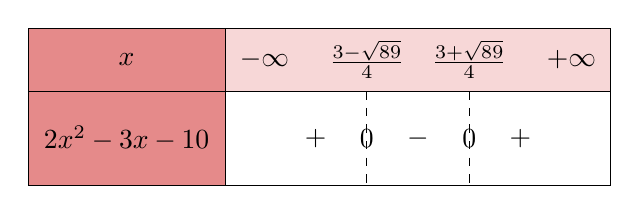
\begin{tikzpicture}
\tikzset{t style/.style = {style = dashed}}
\tikzset{z style/.style = {fill=white,inner sep=.2mm}}
\tkzTabInit[color,lgt=2.5,espcl=1.3,colorC = red7,
colorL = red9,
colorV = red7]%
{$x$ / .8,$2x^2-3x-10$ /1.2}%
{$-\infty$,$\frac{3-\sqrt{89}}{4}$,$\frac{3+\sqrt{89}}{4}$,$+\infty$}%
\tkzTabLine{ , +, z
, -, z
, +, }
\end{tikzpicture}
\end{center}
Οι λύσεις της ανίσωσης είναι το σύνολο $\left(\frac{3-\sqrt{89}}{4},\frac{3+\sqrt{89}}{4}\right)$.
\end{rlist}
\textbf{Ερώτημα Β}\\
Η εξίσωση είναι λογαριθμική και χρειάζεται τους εξής περιορισμούς. Πρέπει
\begin{itemize}
\item $x-2>0\Rightarrow x>2$
\item $x-1>0\Rightarrow x>1$ και 
\item $2x+8>0\Rightarrow 2x>-8\Rightarrow x>-4$
\end{itemize}
Οι περιορισμοί συναληθεύουν όταν $x>2$. Η εξίσωση γράφεται
\begin{gather*}
\ln{(x-2)}+\ln{(x-1)}=\ln{(2x+8)}\Rightarrow\\
\ln{(x-2)(x-1)}=\ln{(2x+8)}\Rightarrow\\
(x-2)(x-1)=2x+8\Rightarrow\\
x^2-2x-x+2=2x+8\Rightarrow\\
x^2-5x-6=0\Rightarrow x=2\ \ \text{ή}\ \ x=3
\end{gather*}
Σύμφωνα με τον περιορισμό πρέπει $x>2$ άρα η δεκτή λύση είναι η $x=3$.\\\\
\askhsh\\
\textbf{Ερώτημα Α}
\begin{rlist}
\item Ο συντελεστής διεύθυνσης της ευθείας $AB$ δίνεται από τον τύπο $a=\dfrac{y_B-y_A}{x_B-x_A}$. Είναι λοιπόν
\[ a=\dfrac{y_B-y_A}{x_B-x_A}=\dfrac{2-7}{-1-4}=\frac{-5}{-5}=1 \]
Η εξίσωση της ευθείας είναι
\begin{gather*}
y-y_A=a(x-x_A)\Rightarrow\\
y-7=1(x-4)\Rightarrow y=x+3
\end{gather*}
\item Αν $a_1,a_2$ είναι οι συντελεστές διεύθυνσης των δύο ευθειών τότε ισχύει
\[ \varepsilon_1\perp\varepsilon_2\Leftrightarrow a_1\cdot a_2=-1=\Leftrightarrow 1\cdot a_2=-1\Leftrightarrow a_2=-1 \]
Έτσι η εξίσωση της θα είναι
\begin{gather*}
y-y_A=a_2(x-x_A)\Rightarrow\\
y-7=-1(x-4)\Rightarrow\\
y-7=-x+4\Rightarrow\\
y=-x+11
\end{gather*}
\end{rlist}
\textbf{Ερώτημα Β}\\
Η εξίσωση της ευθείας $\varepsilon_4$ γράφεται στη μορφή
\[y=\frac{(a-3)x+13}{4}\Leftrightarrow y=\frac{a-3}{4}x+\frac{13}{4}\]
άρα χει συντελεστή διεύθυνσης $a_{4}=\dfrac{a-3}{4}$. Για να είναι οι ευθείες παράλληλες πρέπει
\[ a_3=a_4\Leftrightarrow a+1=\frac{a-3}{4}\Leftrightarrow 4a+4=a-3\Leftrightarrow 3a=-7\Leftrightarrow a=-\frac{7}{3} \]
Για να είναι κάθετες οι ευθείες πρέπει
\begin{gather*}
a_3\cdot a_4=-1\Leftrightarrow (a+1)\cdot\frac{a-3}{4}=-1\Leftrightarrow (a+1)(a-3)=-4\Leftrightarrow\\
a^2-3a+a-3=-4\Leftrightarrow a^2-2a+1=0\Leftrightarrow a=1
\end{gather*}
\askhsh\\
\textbf{Ερώτημα Α}
\begin{rlist}
\item Η γραφική παράσταση της συνάρτησης $g$ τέμνει τον άξονα $x'x$ όταν $g(x)=0$. Οπότε
\[ g(x)=0\Leftrightarrow 5x^2-2x-2=0\Leftrightarrow x=\frac{1+\sqrt{11}}{5}\ \ \text{ή}\ \ x=\frac{1-\sqrt{11}}{5} \]
Άρα τα σημεία τομής είναι $A\left(\frac{1+\sqrt{11}}{5},0\right)$ και $B\left(\frac{1-\sqrt{11}}{5},0\right)$. Επίσης η γραφική παράστση τέμνει τον άξονα $y'y$ όταν $x=0$ άρα
\[ g(0)=5\cdot 0^2-2\cdot 0-2=-2 \]
οπότε το σημείο τομή είναι το $\varGamma(0,-2)$.
\item 
\end{rlist}
\textbf{Ερώτημα Β}
\begin{rlist}
\item Η συνάρτηση $f$ ορίζεται όταν 
\begin{itemize}
\item $x-2\geq 0\Rightarrow x\geq 2$ και 
\item $\sqrt{x-2}\neq 0\Rightarrow x-2\neq 0\Rightarrow x\neq 2$
\end{itemize}
οπότε έχει πεδίο ορισμού το διάστημ $D_f=(2,+\infty)$. Η $g$ αντίστοιχα ορίζεται όταν 
\[x+1\neq 0\Rightarrow x\neq -1\]
άρα $D_g=(-\infty,-1)\cup(-1,+\infty)$. Το κοινό πεδίο ορισμού προκύπτει από την τομή των δύο συνόλων δηλαδή
\[ D=D_f\cap D_g=(2,+\infty) \]
\item Η λύση της εξίσωσης $g(x)=1$ θα αντικατασταθεί στην $f$. Έχουμε λοιπόν
\begin{gather*}
g(x)=1\Leftrightarrow \frac{4}{x+1}=1\Leftrightarrow x+1=4\Leftrightarrow x=3
\end{gather*}
Οπότε για $x=3$ είναι $f(3)=\dfrac{1}{\sqrt{3-2}}=\dfrac{1}{\sqrt{1}}=1$. Ομοίως οι λύσεις της εξίσωσης $f(x)=\frac{1}{3}$ θα αντικατσταθούν στην $g$. Είναι
\[ \frac{1}{\sqrt{x-2}}=\frac{1}{3}\Leftrightarrow \sqrt{x-2}=3\Leftrightarrow x-2=9\Leftrightarrow x=11 \]
Άρα για $x=11$ είναι $g(11)=\dfrac{4}{11+1}=\dfrac{4}{12}=\dfrac{1}{3}$.
\end{rlist}
\askhsh\\
\textbf{Ερώτημα Α}
\begin{rlist}
\item Το σημείο τομής των δύο καμπυλών προκύπτει από τη λύση του παρακάτω συστήματος
\begin{align*}
\begin{cases}
Y=1.100-2.000r\\Y=800+4.000r
\end{cases}&\Rightarrow 1.100-2.000r=800+4.000r\Rightarrow \\&
\Rightarrow6.000r=300\Rightarrow r=\frac{1}{20}=0{,}05=5\%
\end{align*}
Επίσης για $r=0{,}05$ : $Y=1.100-2.000\cdot0{,}05=1.100-100=1000$. Έτσι το σημείο τομής είναι το $(Y,r)=(1000,5\%)$
\item 
\end{rlist}
\textbf{Ερώτημα Β}
\begin{rlist}
\item Η συνάρτηση του κέρδους $\Pi(Q)$ δίνεται από τον τύπο $\Pi(Q)=TR(Q)-TC(Q)$. Είναι λοιπόν
\begin{align*}
\Pi(Q)&=TR(Q)-TC(Q)=50Q-0{,}0005Q^2-\left(2Q+0{,}0025Q^2+101.250\right)=\\&=50Q-0{,}0005Q^2-2Q-0{,}0025Q^2-101.250=-0{,}003Q^2+48Q-101.250
\end{align*}
\item Η παραγωγική δυναμικότητα της επιχείρησης είναι $Q=9.500$ άρα οι παραπάνω συναρτήσεις έχουν πεδίο ορισμού το σύνολο $D=[0,9.500]$. Για την εύρεση του νεκρού σημείου λύνουμε την εξίσωση $\Pi(Q)=0$ οπότε είναι
\begin{gather*}
\Pi(Q)=0\Leftrightarrow -0{,}003Q^2+48Q-101.250=0\\
\varDelta=\beta^2-4a\gamma=48^2-4\cdot(-0{,}003)\cdot(-101.250)=2.304-1.215=1.089
\end{gather*}
οπότε 
\[Q_{1,2}=\frac{-\beta\pm\sqrt{\varDelta}}{2a}=\frac{-48\pm\sqrt{1.089}}{2(-0{,}003)}=\frac{-48\pm 33}{-0{,}006}\]
και τελικά προκύπτει $Q_1=2.500$ ή $Q_2=13.500$ το οποίο όμως ξεπερνά την παραγωγική δυνατότητα άρα το απορρίπτουμε. Έτσι το νεκρό σημείο είναι $Q=2.500$.
\item Για να έχουμε θετικό κέρδος πρέπει \[\Pi(Q)>0\Leftrightarrow -0{,}003Q^2+48Q-101.250>0\] 
Έχοντας υπολογίσει τις ρίζες του τρυωνύμου στο προηγούμενο ερώτημα, προχωράμε στον πίνακα προσήμων:
\begin{center}
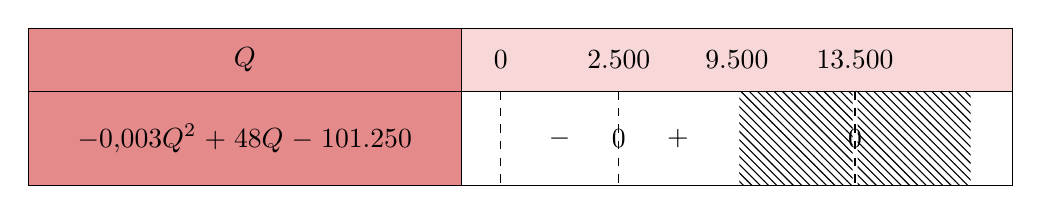
\begin{tikzpicture}
\tikzset{t style/.style = {style = dashed}}
\tikzset{z style/.style = {fill=white,inner sep=.2mm}}
\tkzTabInit[color,lgt=5.5,espcl=1.5,colorC = red7,
colorL = red9,
colorV = red7]%
{$Q$ / .8,$-0{,}003Q^2+48Q-101.250$ /1.2}%
{$0$,$2.500$,$9.500$,$13.500$,}%
\tkzTabLine{ t, -, z
, +, 
, h, z,h}
\end{tikzpicture}
\end{center}
από τον οποίο προκύπτει ότι το κέρδος είναι θετικό όταν $Q\in(2.500,9.500]$.
\end{rlist}
\end{document}
